% Doctorado en Ingeniería
% Creado por: Dr. Esteban Inga Ortega, PhD
% Universidad Politécnica Salesiana
% 20-Abril-2023
%=====================================================
%\documentclass[spanish,es-tabla,ansinew,12pt]{article}
\documentclass[12pt,a4paper]{article}
\usepackage{booktabs}
\usepackage[table,xcdraw]{xcolor}
\usepackage{lmodern}
\usepackage[centertags]{amsmath}
\usepackage[utf8]{inputenc}
\usepackage[T1]{fontenc}
\usepackage[mathscr]{eucal}
\usepackage{ifthen,calc,enumerate}
\usepackage{color}
\usepackage{array}
\usepackage{amsfonts}
\usepackage{textcomp}
\usepackage{amssymb}
\usepackage{amsthm}
\usepackage{newlfont}
\usepackage{graphicx}
\usepackage{subfigure}
\usepackage[hyperindex,colorlinks,breaklinks,pdfstartview=FitH,citecolor=cyan,linkcolor=blue,anchorcolor = green,citecolor=cyan,urlcolor  = blue]{hyperref}
%\usepackage[nonumberlist, numberedsection=true]{glossaries}
\usepackage{rotating}
\usepackage{lscape}
\usepackage{fancyhdr}
\usepackage{colortbl} %color para las tablas
\usepackage{float}
\usepackage{multirow}
\usepackage{enumerate} 
\usepackage{tikz}
\usepackage{url}
\usepackage{pgfplots}
\pgfplotsset{compat=1.18}
\usepackage[upright]{fourier} 
\usetikzlibrary{shapes}
\graphicspath{{Figuras/}}
\usepackage{verbatim}
\usepackage{tikz}
\usetikzlibrary{arrows.meta}
\tikzset{%
  >={Latex[width=2mm,length=2mm]},
  % Specifications for style of nodes:
            base/.style = {rectangle, rounded corners, draw=black,
                           minimum width=4cm, minimum height=1cm,
                           text centered, font=\sffamily},
  activityStarts/.style = {base, fill=blue!30},
       startstop/.style = {base, fill=red!30},
    activityRuns/.style = {base, fill=green!30},
         process/.style = {base, minimum width=2.5cm, fill=orange!15,
                           font=\ttfamily},
}
\usepackage{geometry}
\geometry{
    letterpaper,
    left=3cm,
    right=2.5cm,
    top=2.5cm,
    bottom=2.5cm
}
\renewcommand{\figurename}{Figura}
\renewcommand{\tablename}{Tabla}
\def\refname{Referencias}
%=====================================================
\begin{document}
%----------------------------------------------------------------------
%pat_definiciones
\newcommand\patTitulo
    {Arquetipos de datos semánticos en el diseño UX-UI y modelado del software: mejorando la usabilidad y eficiencia del sistema informático}
\newcommand\patTituloMayus
    {{\textsc \patTitulo}}
\newcommand\patNombre
    {Patricio Michael Paccha Angamarca}
\newcommand\patKeywords
    {Arquetipos de datos semánticos, diseño UX-UI, modelado de software, patrón de diseño de software}
\newcommand\patKeywordsIngles
    {Semantic data archetypes, UX-UI design, Software modeling, Software design pattern}

%portada
     \pagenumbering{arabic}
     \thispagestyle{empty}%
 \begin{titlepage}
    \begin{center}

{{\Large{\textsc{Universidad Politécnica Salesiana}}}} \rule[0.1cm]{16cm}{0.1mm}
\rule[0.5cm]{16cm}{0.6mm}
{\Large{\bf 
    DOCTORADO EN CIENCIAS COMPUTACIONALES 
}}
\end{center}
\vspace{15mm}
\begin{center}
{\LARGE{\bf 
    \patTituloMayus
}}\\
\vspace{6mm}
\end{center}
\vspace{22mm}
\par
\noindent

\begin{figure}
\begin{center}

\includegraphics[scale=0.3]{logoups.png}
\vspace{-0.2cm} 
\end{center}
\end{figure}


\begin{minipage}[t]{0.57\textwidth}
{\large{\bf Director:\\
    Ing. Esteban Inga, Ph.D. \\
{\vskip 5mm} Elaborado por:\\
    \patNombre
}}
\end{minipage}
\hfill
% \begin{minipage}[t]{0.47\textwidth}\raggedleft
%{\large{\bf Elaborado por:\\
%Nombre1 Nombre2 Apellido1 Apellido2}}
%\end{minipage}
\vspace{10mm}
\begin{center}
{\large{\bf 
    Fecha\\
    Julio, 2023 }}%inserire l'anno accademico de la inscritti
\end{center}
\end{titlepage}
%----------------------------------------------------------------------
\newpage
 \thispagestyle{empty}%
     \begin{center}
        \hyphenpenalty=10000\large\uppercase\expandafter{\textbf{
            \patTitulo
        }}
     \end{center}

     \begin{center}
         \vskip2cm
         \hyphenpenalty=10000\large\expandafter{\textbf{
            \patNombre
         }}  \\
         \vfill
         \normalsize 
            Trabajo de inicio de carrera para acceder al Doctorado en Ciencias Computacionales\\
         %\normalsize Mención en Sistemas Eléctricos de Potencia \\
         \vskip1cm
         \normalsize Director\\
         \vskip0.3cm
         \normalsize Ing. Esteban Inga, Ph.D. \\
     \end{center}
     \vfill
    \begin{center}
        
\includegraphics[width=6cm]{logoups.png}\\
        \uppercase\expandafter{Universidad Politécnica Salesiana} \\
        \uppercase\expandafter{DOCTORADO EN CIENCIAS COMPUTACIONALES} \\
        \uppercase\expandafter{Posgrados} \\
        \uppercase\expandafter{Quito, Ecuador} \\
        \uppercase\expandafter{2023}
    \end{center}
%=====================================================
\section{Información General}\label{sec:GeneralInformation}
%=====================================================
\begin{table*}[ht!]
\centering
\begin{tabular}{p{4.5cm}|p{9cm}}
\hline
\textbf{Título}  & \patTitulo \\
\hline
\textbf{Líder} & \patNombre \\
\hline
\textbf{Unidad Académica} & Doctorado en Ciencias Computacionales\\
\hline
\textbf{Entidades Involucradas} & Universidad Politécnica Salesiana  \\ 
\hline
% \multirow{2}{4cm}{\textbf{Entidades Involucradas}} & Universidad Politécnica Salesiana  \\ \hline
\textbf{Lugar de Ejecución} & Quito, Universidad Politécnica Salesiana \\
\hline
\textbf{Fecha de Inicio} &   11-Oct-2023\\
\hline
\textbf{Fecha de Fin} &  11-Dic-2027 \\
\hline
\textbf{Keywords} & \patKeywords \\
\hline
\end{tabular}
\end{table*}
%=====================================================
\section{Título del Proyecto}
%=====================================================
  \patTitulo
%=====================================================
\section{Resumen}
\label{sec:1}
%=====================================================
Text text text text text text text text text text text text text text text text text text text text text text text text text text text text text text text text text text text text text text text text text text text text text text text text text text text text text text text text text text text text text text text text text text text text text text text text text text text text text text text text text text text text text text text text text.

%=====================================================
\section{Descripción}
\label{sec:Description}
%=====================================================
La propuesta de investigación tiene como meta crear una metodología que use arquetipos de datos semánticos según el dominio de negocio para incorporar en el diseño de Experiencia de Usuario (UX) e Interfaz de Usuario (UI) y el modelado de software, con el fin de mejorar la usabilidad y la eficiencia del sistema informático. Se busca el como la integración de arquetipos de datos semánticos
\cite{CardosodeMoraes2016}
\cite{Stavrakos2016}
puede contribuir a crear interfaces de usuario más intuitivas, facilitando la comprensión y la interacción de los usuarios con el sistema
\cite{Feras2022}
\cite{Marco-Ruiz2015a}
. Además, se investigará cómo estos arquetipos pueden mejorar la representación y estructuración de los datos
\cite{Piho2015}
\cite{Marco-Ruiz2015}
\cite{Allones2013}
, lo que permitiría una mayor eficiencia del sistema informático
\cite{Spath2011}
\cite{Epifanio2016}
\cite{Ragozini2017}
\cite{Qanbari2016}
. 
\\\\
La figura \ref{fig:figDescripcion}, muestra de forma visual el flujo de la propuesta de investigación que parte desde la obtención de arquetipos de datos semánticos y son insumos para el diseño UX-UI y el modelado de software, con el fin de mejorar la usabilidad y la eficiencia del sistema informático
\cite{Govinda2015}
\cite{Sari2012}
\cite{Qanbari2016}
. El propósito es comprender cómo la integración de arquetipos de datos semánticos puede contribuir a crear interfaces de usuario más intuitivas, facilitando la comprensión y la interacción de los usuarios con el sistema
\cite{Govinda2015}
\cite{Feras2022}
\cite{Kopanitsa2015}
. Además, se investigará cómo estos arquetipos pueden mejorar la representación y estructuración de los datos e información, lo que permitiría una mayor eficiencia y optimizar la aplicación de software.
\\
\begin{figure}[htb]
  \centering
  {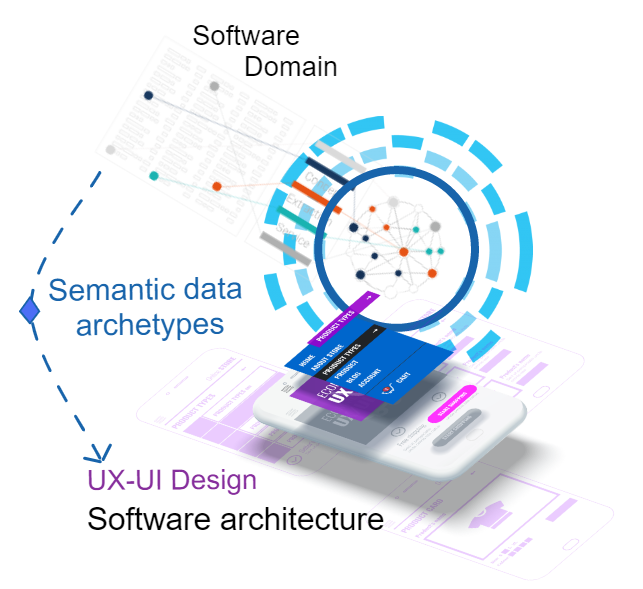
\includegraphics[clip=true,trim= 0cm 0cm 0cm 0cm, width=10cm]{Figuras/figDescripcion.png}}
  \caption{Esquema del arquetipo de datos semánticos en el diseño UX-UI y modelado del software}
  \label{fig:figDescripcion}
\end{figure}
\\
Esta investigación se fundamenta en el uso de métodos cualitativos y cuantitativos, incluyendo pruebas de usabilidad y evaluaciones heurísticas, para valorar y otorgar rigor científico. Estos enfoques permiten evaluar el impacto de los arquetipos de datos semánticos en la experiencia del usuario y la productividad en el desarrollo de sistemas informáticos
\cite{Govinda2015}
\cite{Marco-Ruiz2015}
. Se espera que los resultados de esta investigación contribuyan al avance en el campo de la experiencia de usuario y el modelado de la arquitectura de software, centrándose en la usabilidad y experiencia del usuario. Asimismo, se busca mejorar la eficiencia del sistema informático a través de la implementación de arquetipos de datos semánticos que describen la naturaleza del dominio de negocio
\cite{Duftschmid2010}
\cite{Safina2016}
\cite{Hassan2016813}
. Con esta investigación, se busca aportar conocimientos valiosos para mejorar el diseño y desarrollo de sistemas informáticos, enfocándose en la experiencia del usuario y la optimización de la arquitectura de software.

%=====================================================
\subsection{Formulación del Problema}
\label{sec:2}
%=====================================================
El diseño de Experiencia de Usuario (UX) e Interfaz de Usuario (UI) con el modelado de software son aspectos cruciales en el desarrollo de sistemas informáticos para satisfacer aspectos de usabilidad, expectativas con una experiencia de usuario satisfactoria
\cite{Qanbari2016}
. Sin embargo, la complejidad y la falta de simbiosis entre la representación de datos con el diseño de software pueden obstaculizar la usabilidad y eficiencia del software
\cite{Qanbari2016}
. 
\\\\
Los arquetipos de datos semánticos han surgido como una solución para estructurar y representar datos de manera más comprensible y coherente. Existen evidencias de su utilidad en diversos campos, su aplicación en el diseño UX-UI y el modelado del software aún no ha sido ampliamente explorada y validada
\cite{Qanbari2016}
. Por lo tanto, el problema científico radica en investigar cómo la integración de arquetipos de datos semánticos acorde al dominio de negocio puede mejorar la usabilidad y eficiencia de los sistemas informáticos, y cómo diseñar interfaces de usuario que aprovechen estos arquetipos para una experiencia del usuario intuitiva y satisfactoria
\cite{Allones2013}
\cite{Alomari2020}
\cite{Hassan2016}
. Además, se busca cómo el modelado de software basado en arquetipos semánticos puede agilizar el desarrollo y determinar el modelado adecuado del sistema informático, abriendo la puerta a nuevas posibilidades para la creación de software más efectivo, robusto y centrado en el usuario y sus datos
\cite{Vaclav2017}
\cite{CardosodeMoraes2016}
\cite{Hassan2017}
.
\\\\
Para efecto de la formulación del problema se determina las siguientes variables a considerar para el proceso de investigación.
\\\\
Variables independientes: 
\begin{itemize}
  \item Uso de arquetipos de datos semánticos
  \item Diseño UX-UI
\end{itemize}
Variable dependiente:
\begin{itemize}
  \item modelado de software
\end{itemize}

La contextualización es importante para la selección de los estudios científicos los mismo que deben contener metadata que guarden relación con el objetivo del estudio por lo cual enmarcar la cadena de busqueda es crusial y contempla:
\\\\
Population 
\begin{itemize}
  \item Software architecture 
  \item Software modeling 
\end{itemize}
Income
\begin{itemize}
  \item Semantic data archetypes
\end{itemize}
Outcome 
\begin{itemize}
  \item UX (User Experience) - UI (User Interface) design 
  \item Software Design pattern (Software architecture pattern)
\end{itemize}
Context 
\begin{itemize}
  \item Software industry
  \item Software researchers 
\end{itemize}

Los criterios para la estructuración de los términos de búsqueda se determinan con:
\begin{itemize}
  \item
   Derivar términos clave a partir de la población, intervención, resultados y contexto.
  \item
   Buscar sinónimos para los términos principales planteadas en las preguntas de investigación.
  \item
   Identificar deletreos alternativos, Abreviaciones o simbología de expresiones claves en idioma ingles a valorar en el proceso de busqueda.
\end{itemize}

La cadena de búsqueda es una expresión resultante de la conjunción y combinación terminológica entre las subexpresiones presentadas en la sección de intervención y la sección de resultados expuestos en la sección previa:
\begin{itemize}
  \item  \textbf{  Semantic data archetypes AND (UX/UI design OR design pattern) }
\end{itemize}

El contexto del problema se enmarca en diseño de sistemas informáticos, aplicaciones e interfaces de usuario, experiencia de usuario, entorno de usuarios, desarrolladores y arquitectos de software
\cite{CardosodeMoraes2016}
\cite{Kopanitsa2015}
\cite{Hassan2016813}
.
%=====================================================
\subsection{Hipótesis}
\label{sec:2a}
%=====================================================
La implementación de arquetipos de datos semánticos basados en el dominio de negocio y su vinculación al diseño UX-UI y modelado de los sistemas informáticos tendrá un impacto positivo al mejorar la usabilidad y la eficiencia del software.
\\\\
Esta hipótesis sugiere que una estructura semántica proporcionada por los arquetipos de datos semánticos permitirá una mejor organización y representación de los datos, lo que a su vez facilitará una experiencia de usuario más intuitiva y eficiente desde el modelado del software; pues, otorga al arquitecto de software un patrón de diseño que mejor se ajuste a sus datos. 
\\\\
Para determinar la pertinencia de la hipótesis planteada se determina una etapa de pruebas a través de estudios empíricos, evaluaciones por arquitectos de software, expertos en diseño UX-UI evaluando y realizando mediciones de rendimiento y comparaciones con enfoques de diseño UX-UI tradicionales.

%=====================================================
\subsection{Justificacion del problema}
\label{sec:3}
%=====================================================
La aplicación de arquetipos de datos semánticos en el diseño UX-UI tiene el potencial de mejorar la usabilidad y la eficiencia en el desarrollo de sistemas informáticos al proporcionar una estructura semántica clara y significativa acorde a la información que gestiona para la representación y manipulación de datos
\cite{Stacey2017}
\cite{Marco-Ruiz2015a}
. Sin embargo, hasta el momento, existe una falta de investigación y directrices claras sobre cómo correlacionar de manera simbiótica un arquetipo de datos semánticos en el diseño UX-UI, lo que limita su adopción y el aprovechamiento de sus beneficios potenciales
\cite{Qanbari2016}
.
\\\\
Existe una necesidad creciente de investigar y desarrollar enfoques para diseñar software en el cual se mejoren la usabilidad y la eficiencia en el diseño y desarrollo de los sistemas informáticos
\cite{Spath2011}
\cite{Esposito201610}
\cite{Feras2022}
. Los arquetipos de datos semánticos representan una oportunidad para proporcionar una visión estructural a partir de una semántica clara y significativa de los datos de negocio en el modelado del software, lo que puede facilitar el diseño de interfaces más intuitivas y sistemas informáticos eficientes
\cite{Stacey2017}
\cite{Catalina2008}
\cite{Sari2012}
.
%=====================================================
\subsection{Pertinencia}
\label{sec:4}
%=====================================================
El enfoque de esta propuesta aborda un tema de alta relevancia en el campo de modelado de los sistemas informáticos y el diseño de interfaces de usuario. La mejora de la usabilidad y la eficiencia en el desarrollo de software es un objetivo buscado en la industria del software y en la academia donde no se considera la simbiosis de la aplicación con el arquetipo de datos semánticos en el diseño UX-UI; por lo cual, esta investigación presenta una perspectiva innovadora y prometedora para alcanzar dichos objetivos.
\\\\
La propuesta plateada tiene el potencial de generar beneficios significativos en términos de experiencia de usuario, precisión al diseñar software, eficiencia en el desarrollo modular y calidad de los sistemas informáticos. La aplicación exitosa de arquetipos de datos semánticos según el dominio de negocio durante el diseño UX-UI puede conducir a interfaces más intuitivas, mayor productividad en el desarrollo de software y mejoras en la interacción usuario-sistema.
\\\\
El presente estudio presenta un enfoque innovador y novedoso para el diseño UX-UI y el modelado de sistemas informáticos en base a la integración de arquetipos de datos semánticos del dominio de negocio para proporcionar una perspectiva única para abordar los desafíos actuales en el desarrollo de software y mejorar la usabilidad y la eficiencia en el diseño de interfaces y performances de los sistemas.
\\\\
La tal virtud, la pertinencia de la propuesta radica en la relevancia del campo de estudio, la necesidad de investigación y desarrollo de los potenciales beneficios y avances tecnológicos, y la capacidad de aportar innovación y avance en esta disciplina
\cite{Catalina2008}
. Estos aspectos destacan la importancia y la pertinencia de investigar y explorar la aplicación de arquetipos de datos semánticos en el diseño UX-UI para mejorar la usabilidad y la eficiencia en el desarrollo de software
\cite{Qanbari2016}
.

%=====================================================
\section{Antecedentes}
\label{sec:5}
%=====================================================
El ámbito de la propuesta abarca los Arquetipos de datos semánticos, el diseño UX-UI y el modelado del software. En este contexto, el desarrollo de un sistema informático se fundamenta en la comprensión del dominio de negocio, el cual puede ser abordado desde diversas perspectivas
\cite{Moner2018}
\cite{Kopanitsa2015}
. Thomas Beale destaca que los conceptos del dominio de negocio son directamente codificados en la aplicación y la base de datos
\cite{Cosenz2017}
. En este sentido, los arquetipos juegan un papel crucial al capturar las necesidades de información significativa del sector empresarial mediante un modelo de referencia que incorpora las características estables del dominio
\cite{CardosodeMoraes2016}
\cite{Stavrakos2016}
. Para un análisis más profundo del dominio de negocio, es esencial que los arquetipos de datos semánticos representen la información de manera estructurada y semántica
\cite{Piho2015}
, aprovechando ontologías que brindan un mayor contexto y significado a los datos lo que facilita la interoperabilidad y la comprensión de la información entre diferentes modulo del sistema
\cite{Marco-Ruiz2015}
\cite{Cosenz2017}
\cite{Piho2015}
.
\\\\
Un arquetipo es una combinación estructurada y restringida de datos que estandariza la información al describir y dar significado a un contexto específico a nivel semántico mediante el uso de ontologías
\cite{Kopanitsa2015a}
\cite{Barbieri2013}
\cite{Menárguez-Tortosa2013}
. Coyle, Mori y Huff han destacado que los arquetipos establecen un vínculo terminológico entre códigos, información y aspectos relevantes del dominio
\cite{Barbieri2013}
\cite{Stavrakos2016}
\cite{MartínezCosta2011}
. Sus características clave incluyen la representación semántica, la estandarización y la reusabilidad, lo que facilita la integración de datos y mejora la colaboración en equipos multidisciplinarios, brindando mayor precisión, flexibilidad y facilidad de adaptación. 
\\\\
Los arquetipos de datos semánticos se convierten en el insumo principal para el modelado del software y el diseño de interfaces
\cite{MartínezCosta2011}
\cite{Qanbari2016}
\cite{JansenBosch}
, lo cual optimiza la gestión de información y datos con los que interactúa el usuario
\cite{Batini1992}
\cite{Baruch2017}
. Su aplicación busca mejorar la eficiencia y la usabilidad en el desarrollo de sistemas informáticos y en la experiencia del usuario al interactuar con ellos
\cite{Safina2016}
\cite{CardosodeMoraes2016}
. 
\\\\
El diseño centrado en UX-UI (Experiencia de Usuario e Interfaz de Usuario) mejora la usabilidad al comprender las necesidades y expectativas del usuario
\cite{Kopanitsa2015}
\cite{Cosenz2017}
\cite{Vaclav2017}
. Al diseñar software con una buena usabilidad
\cite{Cosenz2017}
, se logra una mayor facilidad de uso, se reducen los errores y se disminuye la curva de aprendizaje. Esto se traduce en una mayor eficiencia y productividad para los usuarios
\cite{Ferreira2017}
, así como en una experiencia general más satisfactoria
\cite{Vaclav2017}
. 
\\\\
Los principios de diseño UX-UI se basan en crear interfaces centradas en el usuario, que sean simples, claras y consistentes
\cite{Stacey2017}
. También se enfocan en proporcionar feedback y respuesta, jerarquizar visualmente la información, garantizar la accesibilidad y permitir la flexibilidad y personalización
\cite{Upadhyay2023}
\cite{Moner2018}
. Las metodologías de evaluación de la usabilidad incluyen pruebas de usabilidad, evaluación heurística, análisis de tareas, encuestas y cuestionarios, y el uso de eye-tracking
\cite{Epifanio2016}
. Para mejorar la experiencia del usuario, se utilizan técnicas como la iteración y el refinamiento del diseño, la retroalimentación de los usuarios, el seguimiento de métricas de uso y rendimiento, y la participación de los usuarios en el proceso de diseño
\cite{Upadhyay2023}
\cite{Rasmussen2014}
. Estas prácticas buscan crear interfaces intuitivas, eficientes y satisfactorias para los usuarios.
\\\\
En el desarrollo de proyectos de software, los arquetipos de datos semánticos se centran en la solución del problema de diseño considerando las cualidades, necesidades, motivaciones e intereses del usuario que interactuará con los datos o conceptos del dominio
\cite{MartínezCosta2011}
\cite{Klock2017}
\cite{Hassan2017}
. Dado que el comportamiento humano es relativo y cambia con el contexto, los arquetipos evitan hacer suposiciones sobre los usuarios y se enfocan en lograr una experiencia positiva y satisfactoria para ellos
\cite{Martins1990}
\cite{Hassan2016}
. El diseño UX-UI coloca al usuario en el centro del proceso de desarrollo, asegurándose de atender sus necesidades y preferencias de manera efectiva
\cite{Barbieri2013}
\cite{Martins1990}
\cite{Kopanitsa2015}
. Esto implica comprender las metas, tareas y contextos de uso de los usuarios, lo que permite diseñar interfaces que se ajusten a sus necesidades y preferencias
\cite{Gadea2016}
\cite{Pozdniakova2017}
. Al considerar las capacidades, limitaciones y expectativas de los usuarios, se puede crear un software más intuitivo y adaptado a sus requerimientos
\cite{Kopanitsa2015}
\cite{Hassan2017}
. El diseño de interacción humano-computadora (HCI) busca mejorar la naturalidad de la interacción entre usuarios y sistemas, mientras que la experiencia del usuario (UX) se centra en satisfacer las necesidades de los usuarios y crear una experiencia positiva
\cite{Qanbari2016}
\cite{Feras2022}
. 
\\\\
El modelado del software define la estructura y funcionamiento de un sistema informático
\cite{Hassan2016}
\cite{Gadea2016}
. En este contexto, los enfoques y metodologías que utilizan arquetipos de datos semánticos buscan representar la información de manera significativa, otorgándole un sentido contextual y facilitando su integración y reutilización en diferentes partes del sistema
\cite{Ward1987}
\cite{Duftschmid2010}
. Al emplear esta aproximación, se logra una mayor precisión en la definición de las necesidades y expectativas del usuario, reduciendo la probabilidad de errores y retrabajos en el proceso de desarrollo
\cite{Allones2013}
\cite{Mørup2012}
. Así, el uso de arquetipos de datos semánticos en el modelado del software contribuye a un desarrollo más ágil, eficiente y centrado en las necesidades del usuario, mejorando la calidad y la usabilidad del sistema informático resultante.
\\\\
Un arquetipo semántico de datos adecuado al dominio de negocio es esencial en el desarrollo de software para abordar eficientemente todo el proceso
\cite{Govinda2015}
\cite{Gouvas2016}
. Un arquetipo deficiente puede poner en riesgo todo el trabajo realizado, incluso llegando a requerir desechar el proyecto por completo y comenzar de nuevo
\cite{Duftschmid2010}
\cite{Cosenz2017}
. En línea con los principios de desarrollo de software dirigido por modelos, ArchForms representa la unión del modelado semántico de arquetipos y la especificación XForms, conectándose con la biblioteca de componentes RichFaces
\cite{Guo2015}
\cite{Batini1992}
. Esta integración promueve una mejor gestión y especificación de los datos, optimizando así el proceso de desarrollo y asegurando la calidad del proyecto. En esta fase se identificaron las características propias de la arquitectura software, que fueron situadas en los transformadores abstractos, y las características específicas de las plataformas (módulos CodeGen)
\cite{Stacey2017}
\cite{Upadhyay2023}
. 

%=====================================================
\subsection{Alcance del Proyecto}
\label{sec:6}
%=====================================================
El alcance de este proyecto de investigación se enfoca en abordar:
\begin{itemize}
  \item 
   la implementación de arquetipos de datos semánticos en el diseño de Experiencia de Usuario (UX) e Interfaz de Usuario (UI) y como estos puede mejorar la usabilidad y eficiencia de los sistemas informáticos. 
  \item 
  El estudio se centrará en el cómo identificar y desarrollar arquetipos de datos semánticos específicos del dominio de negocio y su impacto en el modelado de software con patrones de diseño. 
  \item 
  El proyecto incluirá la revisión sistemática de la literatura, entrevistas y encuestas para recopilar información sobre las necesidades y expectativas del usuario. Asimismo, se desarrollarán prototipos de software utilizando los arquetipos de datos semánticos propuestos y se llevarán a cabo pruebas empíricas para evaluar la eficiencia y usabilidad del sistema resultante. 
  \item 
  El alcance del proyecto se limitará a aplicaciones de software específicas en un contexto controlado para lograr resultados significativos y generalizables. Se establece como estrategia se considere casos de uso de los arquetipos de datos semánticos dentro de otras áreas para identificación de modelos y metodologías que permitan establecer las generalidades a nivel de patrones de diseño de software.
\end{itemize}
Las restricciones y limitaciones a la presente propuesta son:
\begin{itemize}
  \item 
  No se incluirán arquetipos ni arquetipos de datos relacionadas al modelado o arquitectura de software.
  \item 
  Este proyecto no abarca el diseño de Experiencia de Usuario (UX) e Interfaz de Usuario (UI) cuyas evidencias no estén dentro de mejorar la usabilidad y eficiencia de los sistemas informáticos.
  \item 
  El estudio no abarca elementos considerados como modelamiento, diseño de software u otras ramas o disciplinas como son la arquitectura, la ingeniería de requerimientos e inclusive la arquitectura de software.
\end{itemize}

%=====================================================
\subsection{Estado del Arte}
\label{sec:7}
%=====================================================
En los últimos 5 años, la investigación y el desarrollo en el campo de los arquetipos de datos semánticos han continuado avanzando, con la incorporación de nuevas tecnologías y enfoques para mejorar la eficiencia y usabilidad de los sistemas informáticos
\cite{Hassan2016}
\cite{Zhao2008}
\cite{Rasmussen2014}
. La revisión y análisis de las investigaciones más recientes y relevantes en el campo de la representación semántica de datos usando arquetipos parte de con las ontologías, vocabularios controlados y técnicas de modelado semántico aplicadas a diferentes dominios donde se muestra un creciente interés y avance en el campo de la representación semántica de datos
\cite{Kosti2016}
\cite{Sari2012}
\cite{Chuprina2017}
.
\\\\
El origen de los arquetipos de datos semánticos parte con desarrollo y adopción de estándares y ontologías para la representación de información estructurada, como RDF (Resource Description Framework) y OWL (Web Ontology Language) de la web semántica y el campo de la informática biomédica
\cite{Chuprina2017}
\cite{Chuprina2015}
\cite{Chuprina2016}
. Estos estándares proporcionaron las bases para la representación de datos con significado y permitieron la creación de modelos semánticos en diferentes dominios como en la industria de la salud, uno de los campos donde los arquetipos de datos semánticos han tenido un mayor desarrollo y aplicación es en el contexto de las Historias Clínicas Electrónicas (HCE) y los sistemas de salud interoperables
\cite{Marco-Ruiz2015a}
\cite{alonsobetanzos2016}
\cite{Upadhyay2023}
. 
\\\\
Se han creado ontologías y arquetipos específicos para representar datos clínicos de manera semántica y facilitar la compartición y reutilización de información en el ámbito de la salud
\cite{Upadhyay2023}
\cite{Zhao2008}
. En el campo de la salud, los arquetipos de datos semánticos se han aplicado para la representación estructurada y significativa de la información clínica en Historias Clínicas Electrónicas (HCE) y sistemas de salud interoperables donde los arquetipos han facilitado la compartición de datos médicos entre diferentes instituciones y han permitido una mejor gestión y toma de decisiones clínicas
\cite{Moner2018}
\cite{Alomari2020}
\cite{Rasmussen2014}
. En la industria, los arquetipos de datos semánticos se han utilizado para la representación de información en sistemas de manufactura y control de procesos, mejorando la interoperabilidad y la eficiencia en el intercambio de datos entre diferentes equipos y sistemas
\cite{Marco-Ruiz2015a}
. En el ámbito de la educación, los arquetipos de datos semánticos han sido aplicados para la representación de contenido educativo estructurado y la mejora de la experiencia de aprendizaje en entornos de educación en línea
\cite{Rasmussen2014}
\cite{CardosodeMoraes2016}
\cite{Baruch2017}
.
\\\\
Un arquetipo semántico de datos es fundamental en el desarrollo de software para abordar eficientemente el proceso
\cite{Stavrakos2016}
\cite{Kopanitsa2015a}
\cite{Piho2015}
. ArchForms, como generador extensible, integra el modelado semántico de arquetipos con la especificación XForms, conectándose con la biblioteca de componentes RichFaces
\cite{Piho2014}
\cite{Barbieri2013}
\cite{Menárguez-Tortosa2013}
. Esto optimiza el proceso de desarrollo y asegura la calidad del proyecto
\cite{MartínezCosta2011}
\cite{Martins1990}
\cite{Ward1987}
. Las aplicaciones de ArchForms gestionan la Historia Clínica Electrónica (HCE) basándose en la norma ISO 13606, con formularios que permiten almacenar parcialmente la información
\cite{Mittas2014}
\cite{Eklund2013}
\cite{Kosti2016}
. Una vez completada la introducción de datos, el usuario puede solicitar la generación y almacenamiento de la información como un extracto de la HCE, mejorando la precisión y accesibilidad de los datos médicos
\cite{Chuprina2017}
\cite{Giabbanelli2016}
\cite{Brunner2016}
. Investigaciones también abordan cómo los arquetipos de datos semánticos influyen en la eficiencia y calidad del software en el modelado que son los casos de uso y aplicaciones prácticas de arquetipos de datos semánticos en el diseño de Experiencia de Usuario (UX) e Interfaz de Usuario (UI) en diferentes sistemas informáticos
\cite{Sari2012}
\cite{Dobre2014}
\cite{Chuprina2015}
.
\\\\
Los arquetipos semánticos de datos están experimentando tendencias hacia una mayor interoperabilidad y estándares, integración con tecnologías de inteligencia artificial y procesamiento del lenguaje natural, y su aplicación en el Internet de las cosas (IoT)
\cite{Chuprina2016}
\cite{Ryabinin2015}
\cite{alonsobetanzos2016}
. Sin embargo, se enfrentan a desafíos en la adaptación a nuevos dominios complejos, la integración con sistemas existentes, la seguridad y privacidad de los datos, y la aceptación y adopción por parte de desarrolladores y usuarios
\cite{Sari2012}
\cite{Casey2015}
\cite{Vinoski2007}
. Aunque continúan evolucionando, estos arquetipos muestran un potencial significativo para mejorar la eficiencia y calidad de los sistemas informáticos al estructurar y gestionar datos de manera más semántica; es aquí donde radica la importancia de destacar que la línea de tiempo de los arquetipos de datos semánticos evoluciona y se expande con nuevas investigaciones y desarrollos en diferentes dominios y aplicaciones
\cite{Marco-Ruiz2015a}
\cite{Spath2011}
. 
\\\\
En campo de acción del diseño UX-UI se ha vuelto cada vez más centrado en el usuario, con un enfoque en comprender las necesidades, expectativas y comportamientos de los usuarios para crear experiencias más satisfactorias y atractivas
\cite{Sari2012}
\cite{Govinda2015}
. Desde la década de 1970 se acuña el término "UX" y conjuntamente los principios de diseño centrado en el usuario y la usabilidad comenzaron a surgir con la investigación de pioneros como Donald Norman, quien acuñó el término "Design of Everyday Things" (Diseño de Objetos Cotidianos) en 1988
\cite{Kopanitsa2015}
\cite{Marco-Ruiz2015}
. En los años 80 y 90, se crea un enfoque donde se incorpora la ergonomía y la interacción humano-computadora (HCI) se convirtieron en campos de estudio más establecidos, sentando las bases para el diseño UX-UI
\cite{Epifanio2016}
\cite{Ragozini2017}
. 
\\\\
Durante la última década, con la expansión de la web, la importancia del diseño de interfaces y la experiencia del usuario se hizo más evidente con las grandes compañías tecnológicas como Google y Amazon comenzaron a enfocarse en la usabilidad y la experiencia del usuario como ventajas competitivas tomando fuerza ampliamente su reconocimiento en la industria
\cite{Safina2016}
\cite{Qanbari2016}
\cite{Thiele2016}
\cite{Hassan2016}
. 
En los últimos años con el auge de las aplicaciones móviles y la importancia de la experiencia del usuario impulsaron aún más la necesidad de diseñadores UX-UI para enfocarse en la inteligencia artificial, la realidad aumentada y la realidad virtual y abren la brecha a experiencias más inmersivas y personalizadas para los usuarios anexo a la proliferación de dispositivos móviles y pantallas de diferentes tamaños, el diseño responsivo y multiplataforma se ha convertido en una prioridad para garantizar que las interfaces se adapten de manera óptima a diversos dispositivos y resoluciones
\cite{Gadea2016}
\cite{Pozdniakova2017}
\cite{Klock2017}
\cite{Hassan2017}
.
\\\\
La colaboración entre diseñadores, desarrolladores, expertos en experiencia del usuario y otros profesionales se ha fortalecido, facilitando una integración más fluida entre el diseño UX-UI y el desarrollo de software
\cite{Duftschmid2010}
\cite{Allones2013}
\cite{Mørup2012}
. Esto se complementa con diversas métricas y técnicas para evaluar la experiencia del usuario, lo que permite medir la eficacia de las interfaces y orientar futuras mejoras en el diseño
\cite{Gouvas2016}
\cite{Gopu2016}
\cite{Cosenz2017}
. En este proceso, se han empleado enfoques, técnicas y herramientas probadas para mejorar la experiencia del usuario y agilizar el desarrollo de software, incluyendo la integración de datos semánticos en el diseño de interfaces de usuario
\cite{Guo2015}
\cite{Vaclav2017}
. Esta integración busca mejorar la usabilidad y la experiencia del usuario, lo que a su vez contribuye a una mejor comprensión de los datos y una interacción más efectiva con los sistemas informáticos
\cite{Marco-Ruiz2015}
\cite{JansenBosch}
.
\\\\
La revisión de hallazgos, pruebas empíricas y comparaciones con enfoques tradicionales se ha llevado a cabo mediante el uso de técnicas como recorridos cognitivos y encuestas de evaluación heurística
\cite{Hassan2016813}
\cite{Batini1992}
. Estos análisis han permitido descubrir correlaciones estadísticamente significativas que están influenciadas por las instituciones y patrones de comportamiento presentes en el entorno
\cite{Esposito201610}
\cite{Ferreira2017}
\cite{Feras2022}
. Con base en estas observaciones, el presente proyecto se enfoca en el desarrollo de UX/UI, empleando técnicas de análisis de datos y encuestas para recopilar información sobre las preferencias y expectativas de los usuarios
\cite{Stacey2017}
\cite{Upadhyay2023}
\cite{Zhao2008}
. Esto permitirá ofrecer una experiencia de usuario optimizada y fundamentada en datos
\cite{Gibbs2015}
\cite{Catalina2008}
. El objetivo final de esta propuesta es mejorar la flexibilidad del software, reducir el tiempo de desarrollo y aumentar la productividad de los desarrolladores
\cite{Moner2018}
\cite{Alomari2020}
.

\begin{figure}[ht!]
\centering
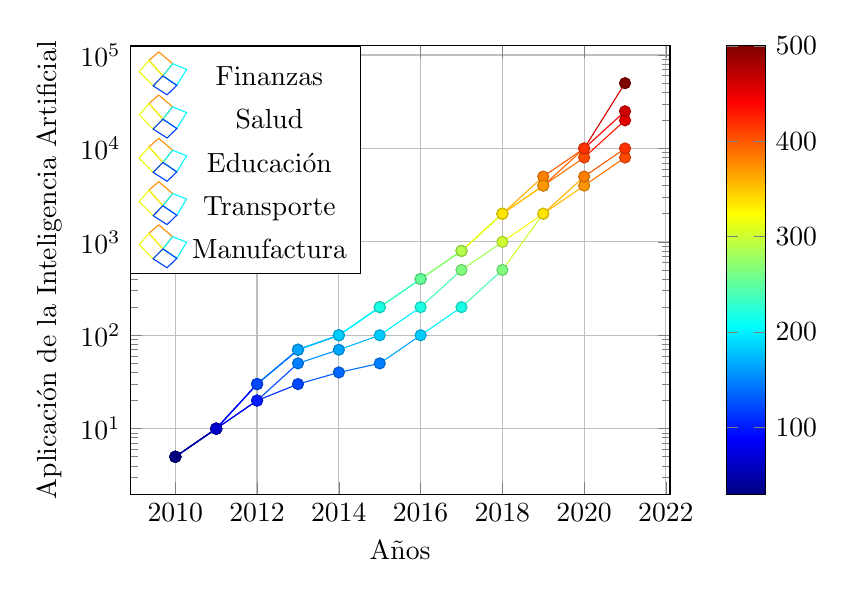
\begin{tikzpicture}
\begin{semilogyaxis}[
colormap/jet,
colorbar,
colorbar style={point meta min=30, point meta max=500, ytick={100,200,300,400,500}},
grid=major,
xlabel=Años,
ylabel=Aplicación de la Inteligencia Artificial,
domain=2010:2021,
x tick label style={/pgf/number format/1000 sep=},
legend style={at={(0,1)},anchor=north west},
]
\addplot+[mark=,solid,scatter,mesh,samples=12,scatter src=y] coordinates
{(2010,5) (2011,10) (2012,20) (2013,30) (2014,40) (2015,50) (2016,100) (2017,200) (2018,500) (2019,2000) (2020,4000) (2021,8000)};
\addplot+[mark=,solid,scatter,mesh,samples=12,scatter src=y] coordinates
{(2010,5) (2011,10) (2012,30) (2013,70) (2014,100) (2015,200) (2016,400) (2017,800) (2018,2000) (2019,4000) (2020,8000) (2021,20000)};
\addplot+[mark=*,solid,scatter,mesh,samples=12,scatter src=y] coordinates
{(2010,5) (2011,10) (2012,20) (2013,50) (2014,70) (2015,100) (2016,200) (2017,500) (2018,1000) (2019,2000) (2020,5000) (2021,10000)};

\addplot+[mark=*,solid,scatter,mesh,samples=12,scatter src=y] coordinates
{(2010,5) (2011,10) (2012,30) (2013,70) (2014,100) (2015,200) (2016,400) (2017,800) (2018,2000) (2019,5000) (2020,10000) (2021,25000)};

\addplot+[mark=*,solid,scatter,mesh,samples=12,scatter src=y] coordinates
{(2010,5) (2011,10) (2012,30) (2013,70) (2014,100) (2015,200) (2016,400) (2017,800) (2018,2000) (2019,4000) (2020,10000) (2021,50000)};
\legend{Finanzas, Salud, Educación, Transporte, Manufactura}
\end{semilogyaxis}
\end{tikzpicture}
\caption{Aumento de las aplicaciones de inteligencia artificial}
\label{fig:4}
\end{figure}

%=====================================================
\section{Objetivos}
\label{sec:8}
%=====================================================
Los objetivos de la propuesta doctoral contemplan aspectos de la metodología y las técnicas para abordar las preguntas de investigación a los arquetipos de datos semánticos que mejoran la usabilidad y la eficiencia en el diseño de UX-UI para el modelado de sistemas informáticos con resultados esperados significativos que aporten al conocimiento científico y la práctica en el campo de la ingeniería de software.
\\
%=====================================================
\subsection{Objetivo General}
\label{sec:9}
%=====================================================
Crear una metodología que facilite la implementación de arquetipos de datos semánticos adaptados al dominio de negocio, permitiendo su integración efectiva en el diseño UX-UI y el modelado de sistemas informáticos. La meta es mejorar significativamente la usabilidad y la eficiencia del sistema informático, proporcionando una experiencia del usuario más intuitiva y efectiva. Esta metodología buscará optimizar la gestión de la información y los datos de negocio relevantes, asegurando una experiencia al usuario mejorada y una mayor productividad en el desarrollo de software, a través de pruebas empíricas y comparaciones con enfoques tradicionales 
\\
%=====================================================
\subsection{Objetivos Específicos}
\label{sec:10}
%=====================================================
\begin{itemize}
  \item 
  Desarrollar directrices y mejores prácticas para la integración efectiva del arquetipo de datos semánticos en el diseño UX-UI, con el fin de mejorar la usabilidad y la eficiencia en el desarrollo de sistemas informáticos.
  \item 
  Evaluar la efectividad y la satisfacción del usuario al utilizar el enfoque de arquetipos de datos semánticos en el diseño UX-UI en comparación con los enfoques tradicionales
  \item 
  Clasificar los arquetipos de datos semánticos que mejoran la usabilidad y la eficiencia en el diseño de UX-UI en el contexto del modelado de sistemas informáticos
\end{itemize}

%=====================================================
\section{Metodología}
\label{sec:11}
%=====================================================
El proceso de investigación aborda una metodología de investigación mixta que combina elementos cuantitativos y cualitativos estructurados en etapas sistémicas:
\begin{itemize}
  \item \textbf{ Método descriptivo: }\\
   Se inicia con la revisión sistemática de la literatura existente sobre arquetipos de datos semánticos, diseño UX-UI, usabilidad y eficiencia en el desarrollo de software. Esto permitirá establecer una base teórica sólida y comprender el estado del conocimiento en el campo de estudio. 
   \item \textbf{ Método exploratorio y experimental: }\\
   La investigación cualitativa comprende entrevistas en profundidad y grupos de discusión con expertos en diseño UX-UI, desarrolladores, arquitectos de software y usuarios avanzados para obtener una comprensión detallada de las percepciones, necesidades y desafíos relacionados con la aplicación de arquetipos de datos semánticos en el diseño y modelado de software. 
   \\
   La investigación cuantitativa para diseñar y aplicar encuestas a una muestra representativa de usuarios para recopilar datos cuantitativos sobre la experiencia del usuario, la eficiencia en el desarrollo de software y la usabilidad de las interfaces basadas en los arquetipos de datos semánticos. 
   \\
   Como parte complementaria de esta etapa comprende el desarrollo de prototipos de sistemas informáticos que integren arquetipos de datos semánticos en el diseño UX-UI para evaluar su efectividad y usabilidad en situaciones reales. 
   \item \textbf{Método analítico sintético:}\\
   Evaluación empírica para evaluar la usabilidad y eficiencia de los sistemas desarrollados con el uso del arquetipo semántico de datos en el diseño de UX-UI. 
   \\
   Análisis de datos recopilados y resultados durante la evaluación empírica al extraer conclusiones significativas y evaluar la efectividad de la propuesta mediante el análisis de datos cualitativos como cuantitativos obtenidos de las entrevistas, encuestas y pruebas con prototipos para identificar patrones, tendencias y correlaciones significativas. 
  \\
   Interpretación de resultados y los hallazgos para responder a las preguntas de investigación y validar si la implementación de arquetipos de datos semánticos mejora la usabilidad y la eficiencia en el desarrollo de software.
\end{itemize}

La figura \ref{fig:figMetodologia}, muestra de forma visual el flujo sistémico ha seguir en la propuesta de investigación que parte con Revisión sistemática de literatura, Investigación exploratoria, Diseño y desarrollo de prototipos, Evaluación empírica y finaliza con el Análisis de datos y resultados. Finalmente se expone la investigación con la presentación de directrices, mejores prácticas y conclusiones que se fundamentan en los resultados obtenidos, desarrollar directrices y mejores prácticas para el diseño de UX-UI utilizando el arquetipo semántico de datos.

\begin{figure}[htb]
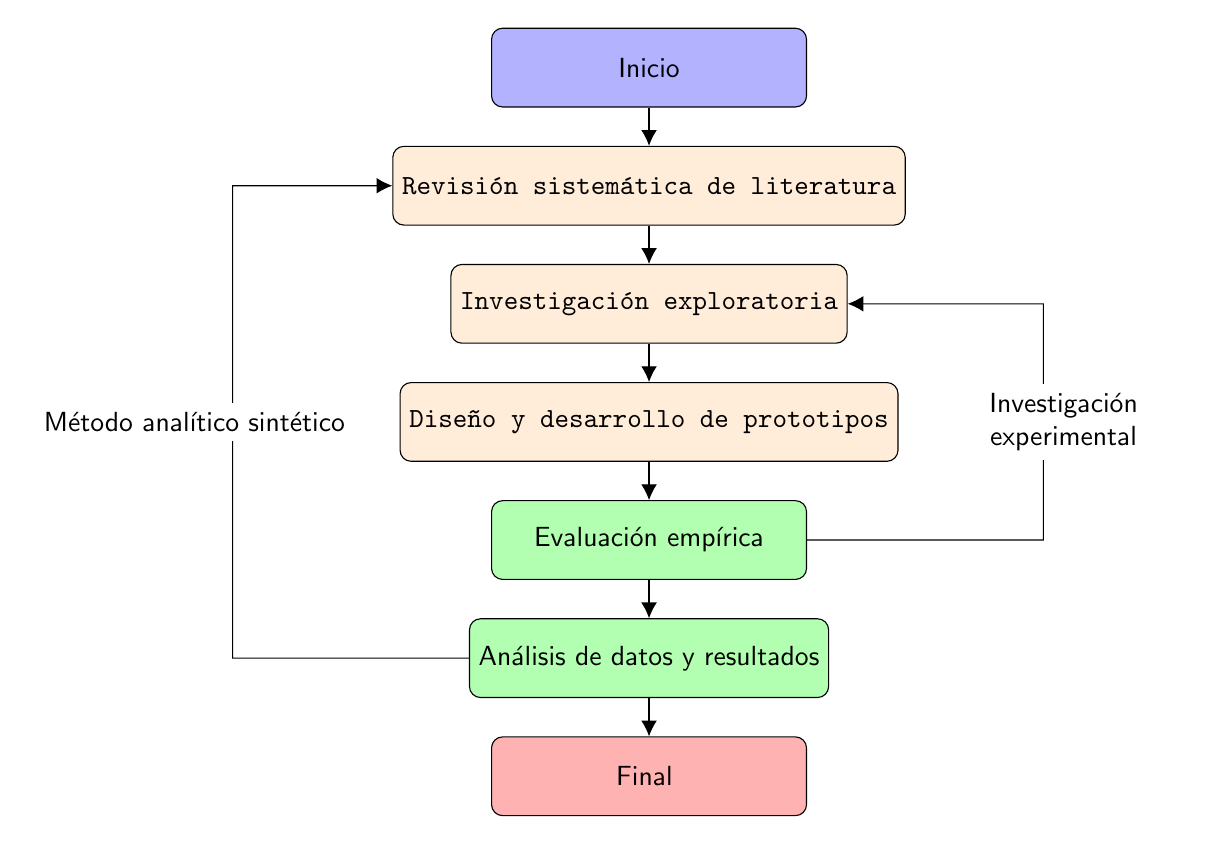
\begin{tikzpicture}[node distance=1.5cm,
    every node/.style={fill=white, font=\sffamily}, align=center]
  % Specification of nodes (position, etc.)
  \node (onStart) [activityStarts]                {Inicio};
  \node (onSLR)   [process, below of=onStart]     {Revisión sistemática de literatura};
  \node (onIE)    [process, below of=onSLR]       {Investigación exploratoria};
  \node (onIEE)   [process, below of=onIE]        {Diseño y desarrollo de prototipos};
  \node (onEE)    [activityRuns, below of=onIEE]  {Evaluación empírica};
  \node (onADR)   [activityRuns, below of=onEE ]  {Análisis de datos y resultados};
  \node (onEnd)   [startstop, below of=onADR]     { Final };     
  \draw[->]     (onStart) -- (onSLR);
  \draw[->]     (onSLR) -- (onIE);
  \draw[->]     (onIE)  -- (onIEE);
  \draw[->]     (onIEE) -- (onEE);
  \draw[->]     (onEE)  -- (onADR);
  \draw[->]     (onADR) -- (onEnd);
  \draw[->] (onEE.east) -- ++(3,0) -- ++(0,2) -- ++(0,1) --                
     node[xshift=1.5cm,yshift=-1.5cm, text width=3cm]
     {Investigación experimental}(onIE.east);
  \draw[->] (onADR.west) -- ++(-3,0) -- ++(0,4) -- ++(0,2) --                
     node[xshift=-1.5cm,yshift=-3cm, text width=4cm]
     {Método analítico sintético}(onSLR.west);
  \end{tikzpicture}
\caption{Metodología mixta aplicada en la Investigación}
\label{fig:figMetodologia}
\end{figure}

%=====================================================
\section{Supervisión y Organización}
%=====================================================
La supervisión bajo la mentoria Académica de Joe Llerena-Izquierdo (ORCID: 0000-0001-9907-7048) Professor of Computer Science, Universidad Politécnica Salesiana. 

%=====================================================
\section{Cronograma del Proyecto}
%=====================================================
Las actividades planificadas para esta propuesta doctoral son:
\clearpage

\begin{table}[H]
\caption{Cronograma de Actividades}
\begin{center}
\begin{tabular}{|p{4.0cm}|c|c|c|c|c|c|c|c|c|c|c|c|c|c|c|c|}
\hline
Actividades &                  \multicolumn{ 4}{|c}{Primer Año} &                 \multicolumn{ 4}{|c}{Segundo Año} &                  \multicolumn{ 4}{|c}{Tercer Año} &                 \multicolumn{ 4}{|c|}{Cuarto Año} \\
\hline
 & $1$ & $2$ & $3$ & $4$ & $1$ & $2$ & $3$ & $4$ & $1$ & $2$ & $3$ & $4$ & $1$ & $2$ & $3$ & $4$ \\
\hline
\hline
\textbf{Actividades Generales}  &  &  &  &  &      &  &  &  &      &  &  &  &      &  &  &  \\ \hline
$~~$Estudios Iniciales    & $\blacksquare$ & $\blacksquare$ & $\blacksquare$ & $\blacksquare$ &      &  &  &  &      &  &  &  &      &  &  &  \\ \hline
$~~$Estado del Arte   &  &  &  &  &     $\blacksquare$ & $\blacksquare$ & $\blacksquare$ & $\blacksquare$ &      &  &  &  &      &  &  &  \\ \hline
$~~$Formulación del Problema   &  &  &  &  &      &  & $\blacksquare$ &  &      &  &  &  &      &  &  &  \\ \hline
$~~$Propuesta de Titulación   &  &  &  &  &      &  &  &  &      &  &  &  &     $\blacksquare$ &  &  &  \\ \hline
$~~$Escritura Trabajo de Titulación      &  &  &  &  &      &  &  &  &      &  &  &  &      & $\blacksquare$ &  &  \\ \hline
$~~$Presentación Oral      &  &  &  &  &      &  &  &  &      &  &  &  &      &  &  & $\blacksquare$ \\ \hline \hline

\textbf{Covertura Rural}      &  &  &  &  &      &  &  &  &      &  &  &  &      &  &  &  \\ \hline
$~~$Definición de Escenarios  &  &  &  &  &     $\blacksquare$ & $\blacksquare$ &  &  &      &  &  &  &      &  &  &  \\ \hline
$~~$Modelo de Despligue        &  &  &  &  &     $\blacksquare$ & $\blacksquare$ & $\blacksquare$ & $\blacksquare$ &      &  &  &  &      &  &  &  \\ \hline
$~~$Tests                    &  &  &  &  &      &  & $\blacksquare$ & $\blacksquare$ &     $\blacksquare$ &  &  &  &      &  &  &  \\ \hline
$~~$Campaña de Simulación     &  &  &  &  &      &  &  & $\blacksquare$ &     $\blacksquare$ &  &  &  &      &  &  &  \\ \hline
$~~$Analisis de Resultados      &  &  &  &  &      &  &  &  &      & $\blacksquare$ & $\blacksquare$ &  &      &  &  &  \\ \hline
$~~$Escritura de Paper        &  &  &  &  &      &  &  &  &      & $\blacksquare$ & $\blacksquare$ & $\blacksquare$ &     $\blacksquare$ &  &  &  \\ \hline \hline

\textbf{Asignación de Recursos} &  &  &  &  &      &  &  &  &      &  &  &  &      &  &  &  \\ \hline
$~~$Defición del Problema       &  &  &  &  &      &  &  &  &     $\blacksquare$ & $\blacksquare$ & $\blacksquare$ & $\blacksquare$ &      &  &  &  \\ \hline
$~~$Modelo de Despliegue        &  &  &  &  &      &  &  &  &      & $\blacksquare$ & $\blacksquare$ & $\blacksquare$ &      &  &  &  \\ \hline
$~~$Tests                    &  &  &  &  &      &  &  &  &      &  & $\blacksquare$ & $\blacksquare$ &      &  &  &  \\ \hline
$~~$Campaña de Simulación     &  &  &  &  &      &  &  &  &      &  &  & $\blacksquare$ &      &  &  &  \\ \hline
$~~$Analisis de Resultados      &  &  &  &  &      &  &  &  &      &  &  & $\blacksquare$ &     $\blacksquare$ &  &  &  \\ \hline
$~~$Escritura de Papers        &  &  &  &  &      &  &  &  &      &  &  & $\blacksquare$ &     $\blacksquare$ & $\blacksquare$ &  &  \\ \hline 
\end{tabular}
\end{center}
\end{table}

%=====================================================
\section{Resultados Previstos}
%=====================================================
Los resultados previstos de esta propuesta doctoral se centran en el diseño e implementación de una metodología para utilizar arquetipos de datos semánticos en el diseño UX-UI y modelado del software, con el objetivo de mejorar la usabilidad y eficiencia del sistema informático, y contribuir al avance en el campo de la experiencia de usuario y el desarrollo de software, tales como:

\begin{itemize}
  \item Desarrollo de una metodología formal para la implementación de arquetipos de datos semánticos en el diseño UX-UI y modelado del software, que permita mejorar la usabilidad y eficiencia del sistema informático.
  
  \item Diseño y desarrollo de arquetipos de datos semánticos acorde al dominio de negocio, para facilitar la representación y gestión de datos en los sistemas informáticos.
  
  \item Evaluación y comparación de la usabilidad y eficiencia del sistema informático antes y después de implementar la metodología y los arquetipos de datos semánticos, utilizando métricas y técnicas de evaluación de experiencia de usuario.
  
  \item Identificación de las ventajas y desafíos en la implementación de arquetipos de datos semánticos en el diseño UX-UI y modelado del software, con el objetivo de proporcionar recomendaciones para futuras aplicaciones.
  
  \item Validación de la propuesta en entornos reales de sistemas informáticos, como aplicaciones de salud, educación o empresas, para demostrar su aplicabilidad y beneficios en situaciones prácticas.
  
  \item Contribución al avance del conocimiento en el campo de la usabilidad, experiencia de usuario y modelado del software, mediante la publicación de los resultados en revistas científicas y la presentación en conferencias y eventos académicos.
  
  \item Mejora en la eficiencia y calidad de los sistemas informáticos, al proporcionar una metodología y enfoque para integrar arquetipos de datos semánticos en el diseño UX-UI y modelado del software.
  
  \item Impacto en la industria y en el campo de la tecnología, al promover el uso de arquetipos de datos semánticos como una herramienta efectiva para mejorar la experiencia del usuario y la eficiencia en el desarrollo de sistemas informáticos.
\end{itemize}

%=====================================================
\section{Estrategias para Presentar Resultados}
%=====================================================
La estrategia que avisoro se enfoca a resaltar logros y beneficios específicos que esta propuesta doctoral aporta en varios sectores de la insdustria de software y académia con múltiples contextos, con el objetivo de compartir el conocimiento generado, generar impacto en la comunidad científica y en el ámbito profesional, y contribuir al avance en el campo de estudio del software, como:

\begin{itemize}
  \item Tesis Doctoral: se expondrán detalladamente los hallazgos, metodologías, conclusiones y recomendaciones derivadas del estudio.
  \item Conferencias y Congresos científicos/académicos : se presenta los resultados relacionados con la informática, diseño UX-UI para comunicar los resultados a través de medios de comunicación y plataformas de divulgación científica.
  \item Revistas Científicas especializadas en informática: se presenta los resultados de la investigacion experimental en el diseño de experiencia de usuario.
  \item Universidades y Centros de Investigación: participar activamente y afiliarse a los grupos de investigación de la Escuela Politécnica Nacional - EPN y Universidad Politécnica Salesiana - UPS para compartir los resultados con investigadores, estudiantes y profesionales interesados en el tema.
  \item Foros y Seminarios: participar activamente en los eventos de divulgación científica organizados por la Escuela Politécnica Nacional - EPN y Universidad Politécnica Salesiana - UPS y otras Entidades.
  \item Organizaciones y Empresas: presentaciones específicas para divulgación científica a empresas o instituciones que utilizan sistemas informáticos y arquetipos de datos semánticos en su trabajo.
\end{itemize}

%=====================================================
\section{Sectores Beneficiados}
%=====================================================
la propuesta doctoral tiene el potencial de beneficiar a múltiples sectores al mejorar la experiencia del usuario y la eficiencia en el uso de los sistemas informáticos mediante la incorporación de arquetipos de datos semánticos, entre los cuales se destaca:

\begin{itemize}
  \item Sector de Desarrollo de Software: Al implementar arquetipos de datos semánticos en el diseño UX-UI y modelado del software, se podrían mejorar los procesos de desarrollo de software, lo que aumentaría la eficiencia y la calidad de los sistemas informáticos creados.

  \item Sector de Tecnología de la Información: La incorporación de arquetipos de datos semánticos podría facilitar la gestión y organización de datos, mejorando la usabilidad de los sistemas informáticos y permitiendo una mayor integración entre diferentes sistemas y plataformas.
  
  \item Sector de Salud: Si la investigación se enfoca en aplicar la propuesta en el ámbito de la salud, los sistemas de registros electrónicos y aplicaciones médicas podrían beneficiarse con una mayor eficiencia y usabilidad, lo que mejoraría la atención al paciente y la gestión de datos médicos.
  
  \item Sector de Educación: Si la propuesta se aplica en el desarrollo de sistemas educativos o aplicaciones de aprendizaje en línea, se podrían mejorar la experiencia del usuario y la eficiencia en el acceso a la información relevante para los estudiantes.
  
  \item Sector de Empresas y Negocios: La mejora en la usabilidad y eficiencia de los sistemas informáticos podría tener un impacto positivo en la productividad de las empresas y en la experiencia del cliente al utilizar sus servicios en línea.
  \end{itemize}
%=====================================================
\section{Grupos de investigación}
%=====================================================
\subsection{Grupo Interno}
\hspace{1cm} 
\textbf{IDE IA GEO CA - Grupo de Investigación de Infraestructura de Datos Espaciales, Inteligencia Artificial y Computación Aplicada}
\subsection{Grupo Externo}
\hspace{1cm} 
\textbf{Grupo de Creación, Aplicación y Gestión en Ingeniería de Software (GI-CreAGSoft) en la Escuela Politécnica Nacional (EPN) }.\\
Grupo de Investigación de "Creación, Aplicación y Gestión en Ingeniería de Software (GI-CreAGSoft)", auspiciado por Consejo del DICC, en sesión del 02 de agosto de 2017, mediante Resolución No. 099.027.02-08-2017.
%=====================================================
\section{Presupuesto}
%=====================================================
Proyección del presupuesto para la propuesta de investigación doctoral.
\begin{table}[ht!]
\caption{Descripción del personal}
\begin{tabular}{|p{1.1cm}|p{1.1cm}|p{1.1cm}|p{1.1cm}|p{1.3cm}|p{1.1cm}|p{1.1cm}|p{1.1cm}|p{1.1cm}|p{1.1cm}|} \hline
Person. & Grado & Func. & Dedic.  & Dedic.  & \multicolumn{4}{|c|}{Recursos} & Total \\ \cline{6-9}
  &   &   & (horas / semana)  &  (\# Meses) & Est. PhD  & UPS & Emp. Privada & Senescyt &  \\ \hline \hline
  Patricio Paccha  & Ing  & Mst Estudiante  & 40 & 48 & - & - & - & 115.2M & 115.2M \\ \hline
  Nombre2 Apellido2  & PhD  & Tutor & 4 & 48 & - & - & 57.6M & - & 57.6M \\ \hline
Total &    &   &   &   &   &   & 57.6M &  115.2M & 172.8M \\ \hline
\end{tabular}
\end{table}

%=====================================================
\begin{table}[ht!]
\caption{Descripción del equipo}
\begin{tabular}{|p{3.4cm}|p{3.4cm}|p{1.1cm}|p{1.1cm}|p{1.1cm}|p{1.1cm}|p{1.1cm}|} \hline
Equipos & Justificación & \multicolumn{4}{|c|}{Recursos} & Total \\ \cline{3-6}
 &   & Est. Mst & UPS & Emp. Privada & Senes cyt &  \\ \hline \hline
Desktop PC 1      & Trabajo en UPS  & -    & 4.0M & - & - & 4.0M \\ \hline
Personal Laptop   & Trabajo General & 5.0M & -    & - & - & 5.0M \\ \hline
Servicios de nube & Trabajo General & 3.0M & -    & - & - & 3.0M \\ \hline
Total           &                 & 8.0M & 4.0M & - & - & 12.0M \\ \hline
\end{tabular}
\end{table}

%=====================================================
\begin{table}[H]
\caption{Síntesis}
\begin{tabular}{|p{7.0cm}|p{1.1cm}|p{1.1cm}|p{1.1cm}|p{1.1cm}|p{1.1cm}|} \hline
Item & \multicolumn{4}{|c|}{Recursos} & Total \\ \cline{2-5}
  & Est. Mst. & UPS \\ \hline \hline

Personal          & -    & -    & 57.6M & 115.2M & 172.8M \\ \hline
Software          & -    & 7.0M & -     & -      & 7.0M   \\ \hline
Equipamiento      & 8.0M & 4.0M & -     & -      & 12.0M  \\ \hline
Materiales        & 3.0M & 1.0M & -     & -      & 4.0M   \\ \hline
Bibliografía      & 1.5M & 2.0M & -     & -      & 3.5M   \\ \hline
Publicaciones     & 2.0M & 3.0M & -     & -      & 5.0M   \\ \hline
Viajes            & 5.0M & 10.0M& -     & 22.0M  &37.0M   \\ \hline
Trabajo de Grado  & -    & 7.0M & -     & -      & 7.0M   \\ \hline
Total             &19.5M & 34.0M& 57.6M & 137.2M & 248.3M \\ \hline
\end{tabular}
\end{table}


%=====================================================
\section{Propiedad Intelectual}
%=====================================================
Los derechos de autor moral pertenecen al estudiante de doctorado y al asesor del proyecto y a cualquier persona que haga una contribución intelectual original, durante el proceso o en el resultado final del proyecto. El estudiante de doctorado y el asesor deben ser el autor y coautor de todas las publicaciones nacionales e internacionales generadas por el proyecto. La apariencia de otras personas depende de la calidad de la colaboración recibida. Los derechos de propiedad intelectual se asignan a la Universidad Politécnica Salesiana. 
\\
\bibliographystyle{IEEEtran}
\bibliography{Referencias.bib}
\vfill
\end{document} 
